The study of dynamical systems is traditionally thought to have begun with the publication of "New methods of Celestial Mechanics" by Poincar\'e and expanded with the work of Lyapunov into a theory of the stability of dynamical systems. It was not until the 1960s however that the use of chaos and stability theory exploded across disciplines\autocite{Aubin2002}. 

Dynamics are typically an unnecessary tool when studying the paths of chemical reactions. Their value became apparent however, when Belousov and later Zhabotinsky released published their work on an oscillatory reaction, a reaction that would later come to be known as the BZ reaction\autocite{Winfree1984}. Cycles were also known to exist in the biochemical realm with many famous pathways in organisms such as the Krebs cycle and Calvin cycle; however the BZ reaction was developed to create an inorganic analogue to the Krebs cycle. The development of this cycle allowed for a relatively easily replicable cyclic reaction with with easily measurable indicators of the progress of the reaction. 

The study of dynamical chemical systems has since expanded to a variety of other mechanisms such as self-replicating molecules\autocite{Beutel2007} in addition to studying fractal patterns and dimensionality involved in electrochemical deposits and flame patterns. Despite the fairly wide range of background information required to set up these different models, the underlying mathematical theory used to study these models is identical which has contributed to the wide range of interdisciplinary work performed by theorists in the field.
\section{Background on Dynamical Systems}
Traditional dynamical systems are modelled in continuous time as a system of ordinary differential equations. These systems typically treat time as the singular independent variable and solve for the evolution of one or more variables in terms of time. A classic continuous time dynamical system is the simple pendulum which allows one to model the movement of a pendulum in space in terms of time. This model uses a variety of simplifying assumptions in order to reduce the problem of the pendulum into a single variable function, holding the length of the pendulum and acceleration due to gravity constant.
\begin{equation}
    \frac{d^2}{dt^2}+\frac{g}{L}\sin\theta=0
\end{equation}
Most  attempts  at  modelling  real-world  systems  however  require  the  use  of  multiple dependent variables in order to effectively model.  However, as the amount of variables increases, the complexity of the model increases.  Modelling and $n$-body system acting on each other gravitationally is of obvious interest in astronomy; however, it was quickly found  that  although  a  1  and  2  body  system  were  relatively  simple  to  solve  for,  the introduction of a third body caused significant complications.  The 3-body system is in fact what Poincar\'e studied in order to develop a theory of chaotic deterministic systems\autocite{Poincare1993}.

That is not to say that these systems cannot arrive at ordered solutions.  Although continuous time systems require a minimum of 3 variables in order for chaos to arise, there are typically windows of order in chaotic regimes that allow for stable, oscillatory behavior. The BZ-reaction is still being actively studied and is known to be actually highly complex but is often reduced into 7 primary sub-reactions\autocite{Field1986}. A great deal of the work involved in studying dynamical systems is actually on finding ways to simplify models in order to arrive at more mathematically tractable systems. The BZ-reaction has been simplified to a 3-variable system that still provides the complex periodicity and chaotic behavior characteristic of the model\autocite{Gyorgyi1992}.

Although many processes in the real-world are more intuitively interpreted as operating as a continuous time  function, there are many  occasions where it is possible and  in fact beneficial to think in a discrete-time sense. The prevalence of this type of system varies depending on the exact field of study; however, it is important to note that when computationally modelling continuous time systems, it is impossible for computers to truly operate with continuous variables and thus even these systems are reduced to technically discrete models.

Population dynamics are frequently analyzed as a discrete time system as opposed to continuous time. It is often of more practical use to interpret $t= 0,1,2,3,...$ as the change in population per year or per season as opposed to determining the change in population over infinitesimally small changes in time. In terms of technique, many of the mathematical principles used in analyzing dynamic systems in continuous time apply to discrete time systems; however, it would be a mistake to assume the two were identical. An important distinction between the two is the nature by which chaos can occur. As described previously, a continuous time system requires 3 or more dependent variables in order for chaos to occur. A discrete time system only requires 1 variable in order to display the same type of chaotic behavior.

The systems discussed throughout this paper will be of the discrete variety due to their nature. Laws pertaining to the physical world are scalable to the infinitesimal degree which allows for their use in continuous models. Economic models do not have a basis in physical laws. It is also important to note that, due to the complexity involved in the human behavior that economic models are trying predict, the exact numerical values of the model are typically of minor concern. The general behavior of the model is significantly more valuable in order to determine the effects of an economic assumption.

The logistic map is regarded as the prototypical chaotic discrete time mapping. The logistic function, which the logistic map is based off of, was developed to study population dynamics but actually garnered widespread use in other disciplines such as the study of autocatalytic reactions, computer science, statistics, and economics\autocite{Kavanagh1934}.
\begin{equation}
    \frac{d}{dx}f(x)=f(x)(1-f(x))
\end{equation}
The logistic function has 2 equilibria or points where the derivative of the function is 0. $f(x) = 0$ is an unstable equilibrium but $f(x)=1$ is a stable equilibrium point which means that other points on the function will tend towards this equilibrium overtime.  This can be realized by solving for the derivative of the function at points when $f(x)\in(0,1)$ which is universally positive and $f(x)\in(1,\infty)$ which is negative. Integrating the differential equation gives the general form equation:
\begin{equation}
    f(x)=\frac{e^x}{e^x+C}
\end{equation}
This function gained prominence due to its rapid, exponential growth when $f(x)$ is low and its slow, linear decaying to non-existent growth as population increases.  Used by notable mathematicians operating in the field of population dynamics such as Verhulst, Pearl, and Lotka, the model continues to be widely used today and is often the basis upon which other modifications are applied\autocite{Zwanzig1973}.

\begin{equation}
    x_{t=1}=\mu x_t(1-x_t)
\end{equation}
The logistic map is a difference equation model popularized by Robert May as a discrete time analogue to the logistic function\autocite{May1976}. When interpreted in the biological context, $x_t$ refers to the ratio of the population at time $t$ compared to the maximal population, thus the mapping is bounded between 0 and 1. Here we see intuitively the major difference between difference equation and differential equation based systems. Differential equations solve for the derivative of a variable with respect to time in terms of the variable, difference equations solve for the actual state of the variable in the successive state provided we know the state of the variable in the previous time period. Much like how differential equations can be of higher order with the introduction higher order derivatives, a difference equation can also be of higher order by including more time periods in the function for the state of the variable which is valuable in a variety of the models discussed later.

Much like how the equilibrium points were solved for in the differential equation, difference equations also have equilibrium points where $x_{t+1}=x_t$. Interestingly, unlike the logistic function, there does not exist a fixed point at $x_t=1$ as this would result in $x_{t+1}=0$. Solving for the fixed points, we have:
\begin{equation}
    x_{t+1}=x_t=0,\frac{\mu-1}{\mu}
\end{equation}

The stability of a fixed point is again dependent on the derivative of the function; however, there are differences in the details of our analysis. Treating $f(x)=x_{t+1}$, we see the derivative of the logistic map is:
\begin{equation}
    f^\prime(x)=\mu(1-2x)
\end{equation}
For reasons that will become clear later, the stability of a point on the map requires that $|f^\prime(x)|<1$. Solving for when this is true for our two fixed points, we see that $\mu<1$ provides stability for the origin fixed point and $1<\mu<3$ gives stability for the non-zero fixed point. Thus, provided the parameter $\mu$ satisfies either of the conditions set previously, it will converge to one of the fixed points in a relatively small, finite amount of iterations. 

This behavior can be visualized using a cobweb diagram. This diagram consists of 3 primary elements: a plot of the mapping, a \SI{45}{\degree} line, and a plot of the variable's trajectory. An example of a cobweb diagram can be seen in Figure \ref{log_fixed_cob}. This diagram shows the trajectory of $x$ starting at a value of 0.1 when there is a stable, non-trivial fixed point.

\begin{figure}
    \centering
    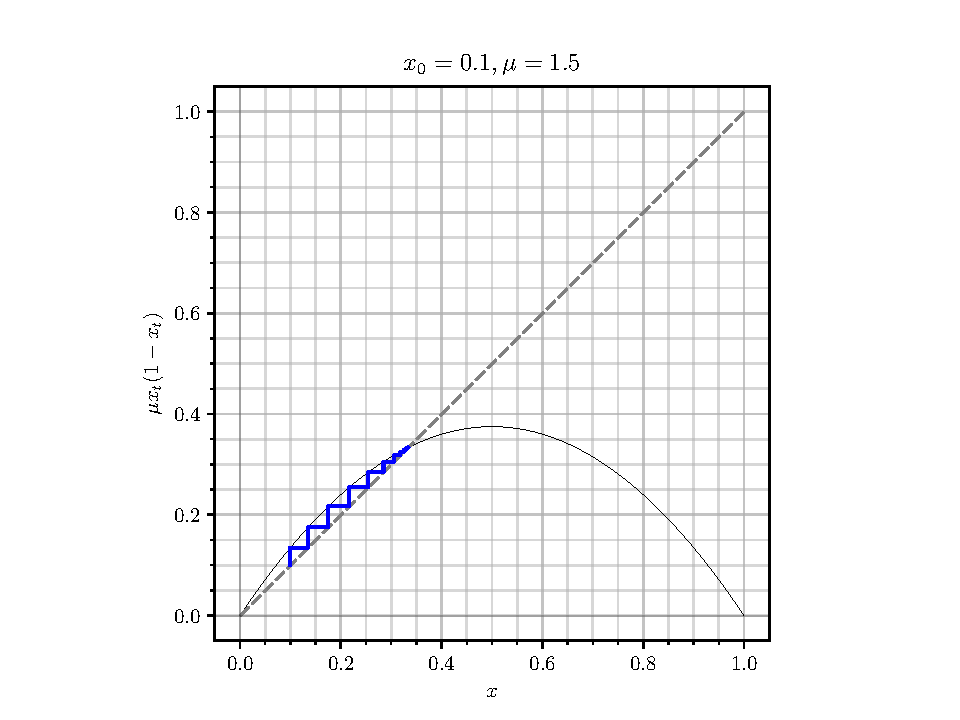
\includegraphics[height=0.4\textheight]{./logistic/fixed_cob.pdf}
    \caption{Cobweb plot of the logistic map setting $\mu=1.5$ and $x_0=0.1$. The trajectory asymptotically approaches the equilibrium point of $\frac{1}{3}$.}
    \label{log_fixed_cob}
\end{figure}
The \SI{45}{\degree} line is defined as the line where $x_t=x_{t+1}$ which is useful for determining the result of successive iterations. Beginning from the point $x_0$, we can then determine what point $x_1$ wll be via the mapping. We can then look horizontally to the \SI{45}{\degree} line until we intersect with it. The $x$-coordinate of this intersection point is equivalent to the result of the mapping of the previous iteration, thus using this new point will allow us to determine the result of the next iteration of the function. This process can be repeated ad infinitum; however, the result will soon prove uninteresting for stable points and orbits as the trajectory will converge and repeat its behavior.

The reason the logistic map is so frequently studied is because of its ability to exhibit complex behavior beyond a stable equilibrium solution. Once $\mu>3$, the mapping enters a cyclic region. Much like how fixed points could be solved for by identifying where $x_{t}=x_{t+1}$, stable oscillatory points can be found by solving for the equilibrium points of higher iterations of the function. A 2-cycle will be such that $x_{t}=x_{t+2}\neq x_{t+1}$ for example and the stability of a such a cycle can be found using the same methodology as described previously. 
\begin{figure}
    \centering
    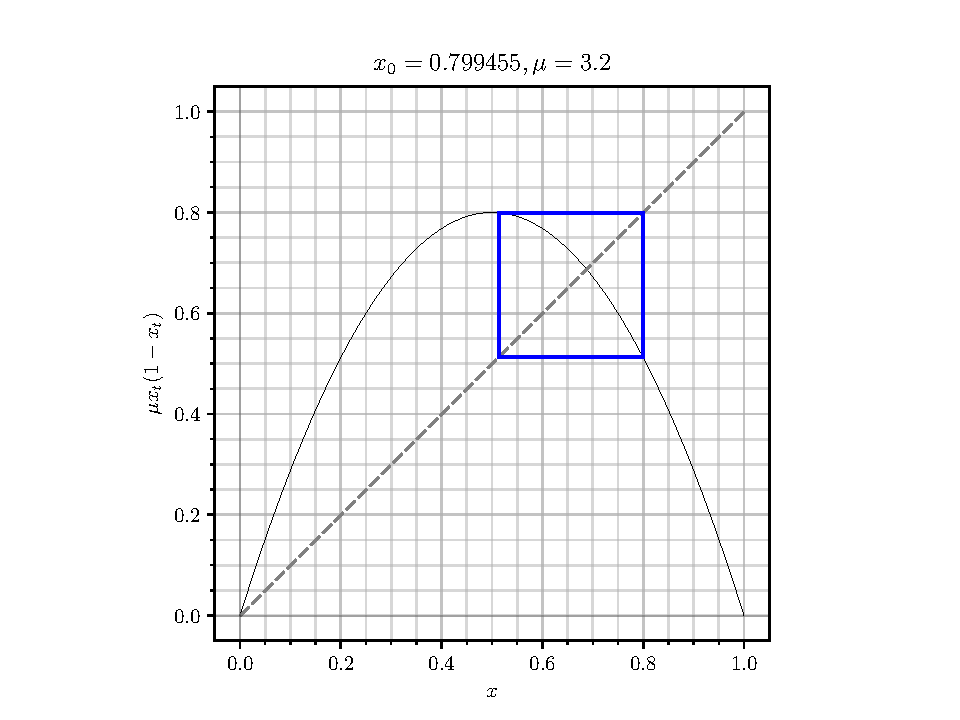
\includegraphics[height=0.4\textheight]{./logistic/2-cyclic_cob.pdf}
    \caption{2-period cycle of the logistic map showing only the cyclic behavior.}
    \label{log_cyclic_cob}
\end{figure}
The logistic map also provides a mechanism to more quantitatively describe what it means for a system to be chaotic. The Lyapunov exponent, named after one of major driving forces in the development of stability analysis, is used to measure the effect of small perturbations in initial conditions on the trajectory of the variable\autocite{Puu2003}. Conceptually, the logistic map and the systems discussed in this paper are determinisitic. However, chaotic systems have highly divergent trajectories with even small changes in their initial conditions; thus knowing approximately what the initial conditions are does not provide approximate information on the trajectory of the variable. 
\begin{figure}
    \centering
    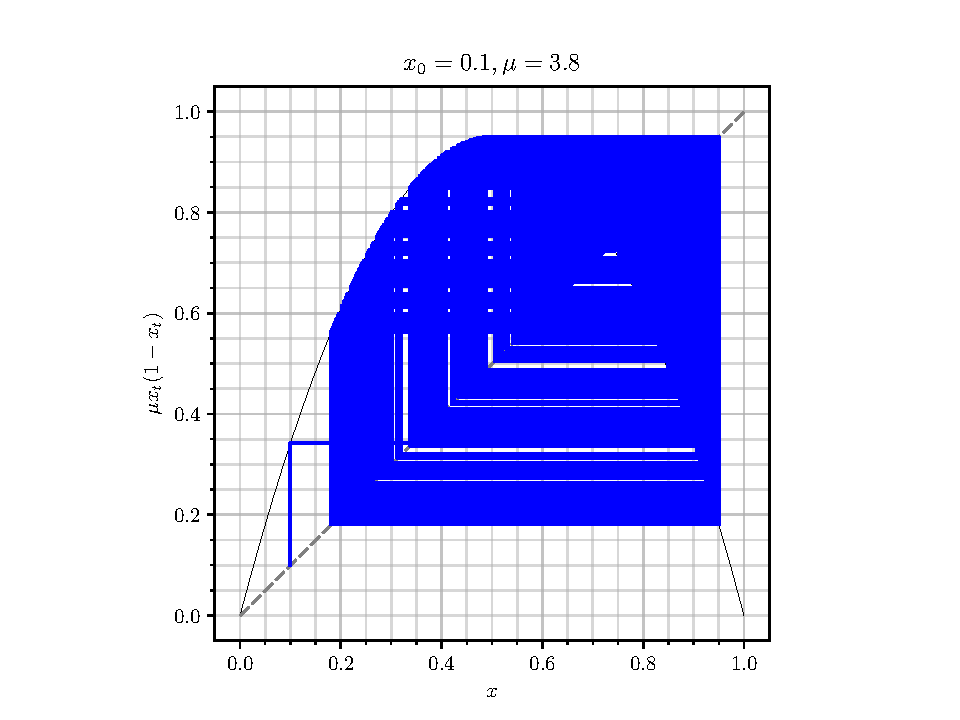
\includegraphics[height=0.4\textheight]{./logistic/chaos_cob.pdf}
    \caption{Chaotic behavior in the logistic map.}
    \label{log_chaos_cob}
\end{figure}

In order to quantify this, we begin by taking the absolute value of the derivative of the function as this allows us to effectively magnify the effect of an infinitesimal change in the intial conditions. We then take the natural logarithm of this derivative in order to measure the exponential rate of separation of trajectories. Finally, we take the average separation over an arbitrarily high number of iterations $n$ as exponential separation is not necessitated over all phase space. This gives us a the equation:
\begin{equation}
    \lambda_n(x_0)=\frac{1}{n}\sum^{t=n}_{t=1}\ln\lvert f^\prime(x_{t-1})\rvert
\end{equation}
where $\lambda_n(x_0)$ is the lyapunov exponent for a given intial point when allowed to run for $n$ iterations. The true value of the lyapunov exponent is the limit of the infinite series as $n\rightarrow\infty$ divided by $n$; however, the complexity of these maps often makes it practically impossible to analytically solve for the limit. By choosing arbitrarily high values of $n$ though, it is possible to achieve better approximations at the expense of computational time. It is also important to note that, although the lyapunov exponent is a function of the initial condition, as long as the initial state is not in some stable fixed point or cycle, the trajectories will follow that of the chaotic attractor, thus the value of the lyapunov exponent should be mostly consistent regardless of the choice of initial conditions.
\begin{figure}
    \centering
    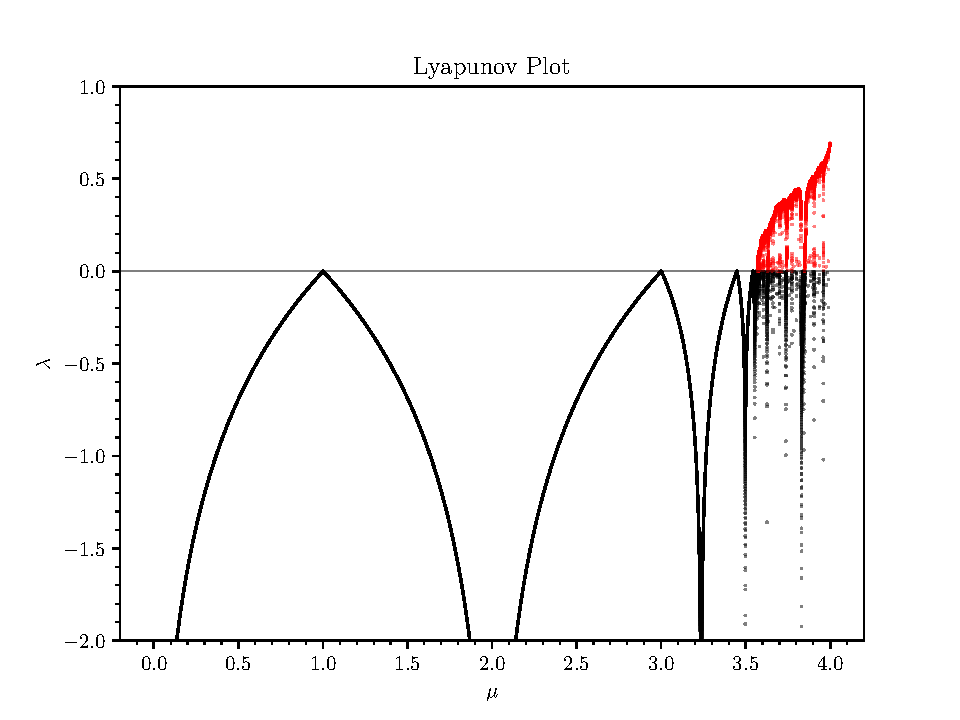
\includegraphics[height=0.4\textheight]{./logistic/lyapunov.pdf}
    \caption{Lyapunov exponent plotted against $\mu$ for the logistic map. Initial value of 0.1 is used. Red denotes regions where $\lambda\geq0$, black denotes regions where $\lambda<0$.}
    \label{log_lyapunov}
\end{figure}

Another way visually see the behavior is with a bifurcation diagram. This diagram shows the longterm behavior of the variable for a given variable. Figure \ref{log_bifurcation} qualitatively shows the behavior described previously. For parameter values between 0 and 1, we see the origin fixed point is stable. For parameter values between 1 and 3, their is still a single fixed point that is monotonically increasing; however, we can also clearly see the beginning of the 2-period cycle once the parameter exceeds 3. It is difficult however, to determine when predictable higher-order cyclic behavior ends and chaotic behavior begins via qualitative observation of the bifurcation diagram. The benefit of the bifurcation diagram is that it allows us to see both where the bifurcation points are and what behavior the bifurcation points signify. Bifurcation points are 
where where infinitesimally small quantitative changes in the parameter induce significant qualitative or topological change in the behavior of the mapping such as the transition from a stable fixed point to a 2-period cycle. 
\begin{figure}
    \centering
    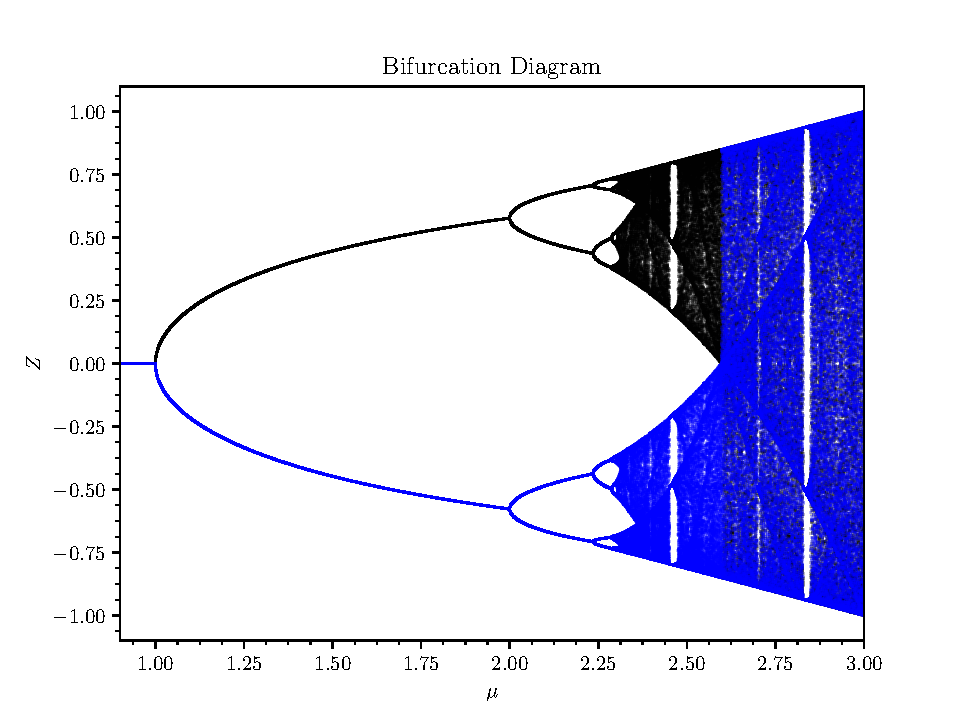
\includegraphics[height=0.4\textheight]{./logistic/bifurcation.pdf}
    \caption{Bifurcation diagram plotting $x$ against $\mu$ for the logistic map.}
    \label{log_bifurcation}
\end{figure}

Research on the logistic map and other iterated maps has shown the existence of what is called Feigenbaum's constant. This constant can be found by observing the behavior of the periodic cycles of the map. The interval of stability decreases and the ratio of subsequence intervals actually approaches a limit $\delta\approx4.6692$\autocite{Puu2003}. All other topologically similar maps with a single local maximum share this Feigenbaum constant. Once the mapping exceeds this constant, chaos occurs which allows for another method to determine precisely where chaotic behavior occurs. 

It is also beneficial to point out that another mechanism exists for cyclic behavior to exist. The previously described method involved taking a mapping and solving for the stability of its double iteration. This allows for $2n$-period stability cycles to exists. However, there does exist odd-ordered cycles such as the $3$ cycle; however, it occurs as a window of order in the region of chaos. These windows can be seen in Figure \ref{log_lyapunov} where the Lyapunov exponent dips into the negative region past the chaotic bifurcation point. These bifurcation points are known as tangent bifurcations
\begin{figure}
    \centering
    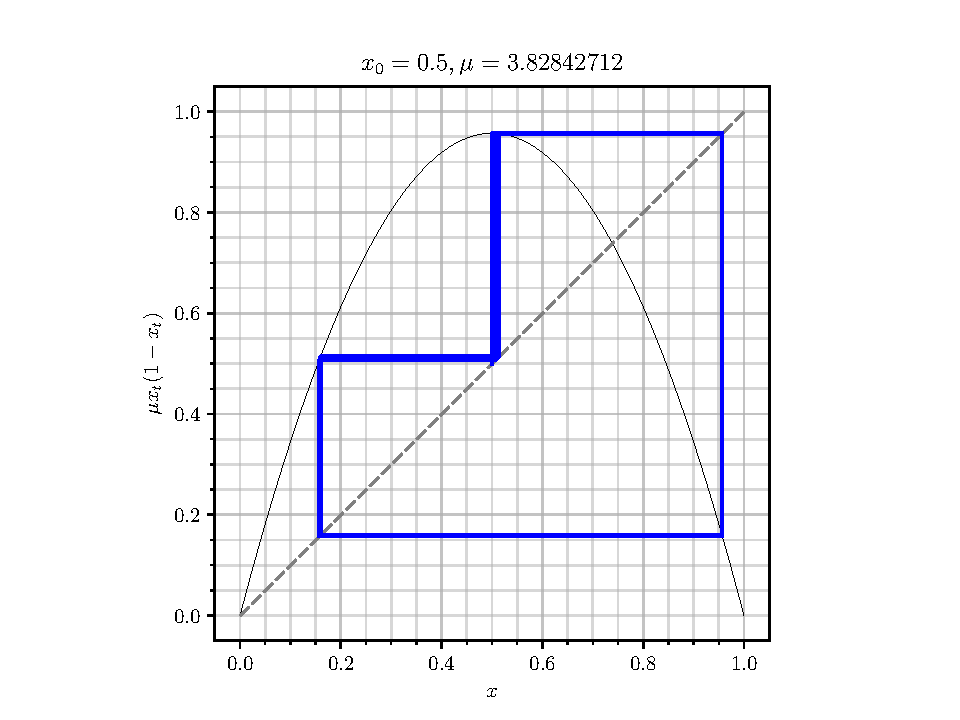
\includegraphics[height=0.4\textheight]{./logistic/3-cyclic_cob.pdf}
    \caption{3-period cycle of the logistic map showing only the cyclic behavior.}
    \label{log_3-cyclic_cob}
\end{figure}
This also allows us to use Sharkovsky's Theorem, which states that any continuous mapping with a 3-period cycle must also have every $n$-period cycle for every $n\in\mathbb{Z}$.\autocite{Puu2003} A variety of other mathematical techniques exist to study the dynamics of difference equation mappings but these will be covered more specifically when used for the specific case. 



